\begin{frame}{VOLE from a GGM tree}
  \begin{center}
    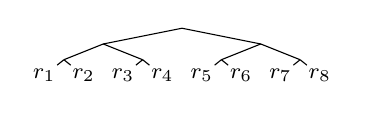
\begin{tikzpicture}[
      level 1/.style = {
        level distance   = 2mm,
        sibling distance = 20mm
      }, level 2/.style = {
        level distance   = 2mm,
        sibling distance = 10mm
      }, level 3/.style = {
        level distance   = 2mm,
        sibling distance = 5mm
      }
    ]
      \tikzset{leaf/.style={circle,inner sep=1pt,outer sep=0pt,font=\footnotesize}}
      \coordinate
        child { coordinate
          child { coordinate
            child { node[leaf] {$r_1$} }
            child { node[leaf] {$r_2$} }
          }
          child { coordinate
            child { node[leaf] {$r_3$} }
            child { node[leaf] {$r_4$} }
          }
        }
        child { coordinate
          child { coordinate
            child { node[leaf] {$r_5$} }
            child { node[leaf] {$r_6$} }
          }
          child { coordinate
            child { node[leaf] {$r_7$} }
            child { node[leaf] {$r_8$} }
          }
        }
      ;
    \end{tikzpicture}
    \vspace{1em}\pause
    $$u=\sum_{i=1}^{2^n}r_i\in \mathbb{F}_2\qquad v=-\sum_{i=1}^{2^n}r_i\cdot i\in \mathbb{F}_{2^n}$$
    $$\Delta=j^*\in \mathbb{F}_{2^n}$$
    \vspace{1em}\\\pause
    Reveal all $r_1,\ldots,r_8$ except $r_{j^*}$:
    $$q=\sum_{i=1}^{2^n}r_i\cdot(j^*-i)=u\cdot\Delta+v\in \mathbb{F}_{2^n}$$
  \end{center}
\end{frame}
